\documentclass[12pt,border=1mm]{standalone}
\usepackage[utf8]{inputenc}
\usepackage[usenames,x11names]{xcolor}
\usepackage[x11names]{xcolor}
\colorlet{ctrlcol}{DeepSkyBlue1}

\usepackage{tikz}
\usetikzlibrary{circuits.logic.IEC}
\usetikzlibrary{arrows,arrows.meta}
\usetikzlibrary{calc,decorations.markings}

\begin{document}
	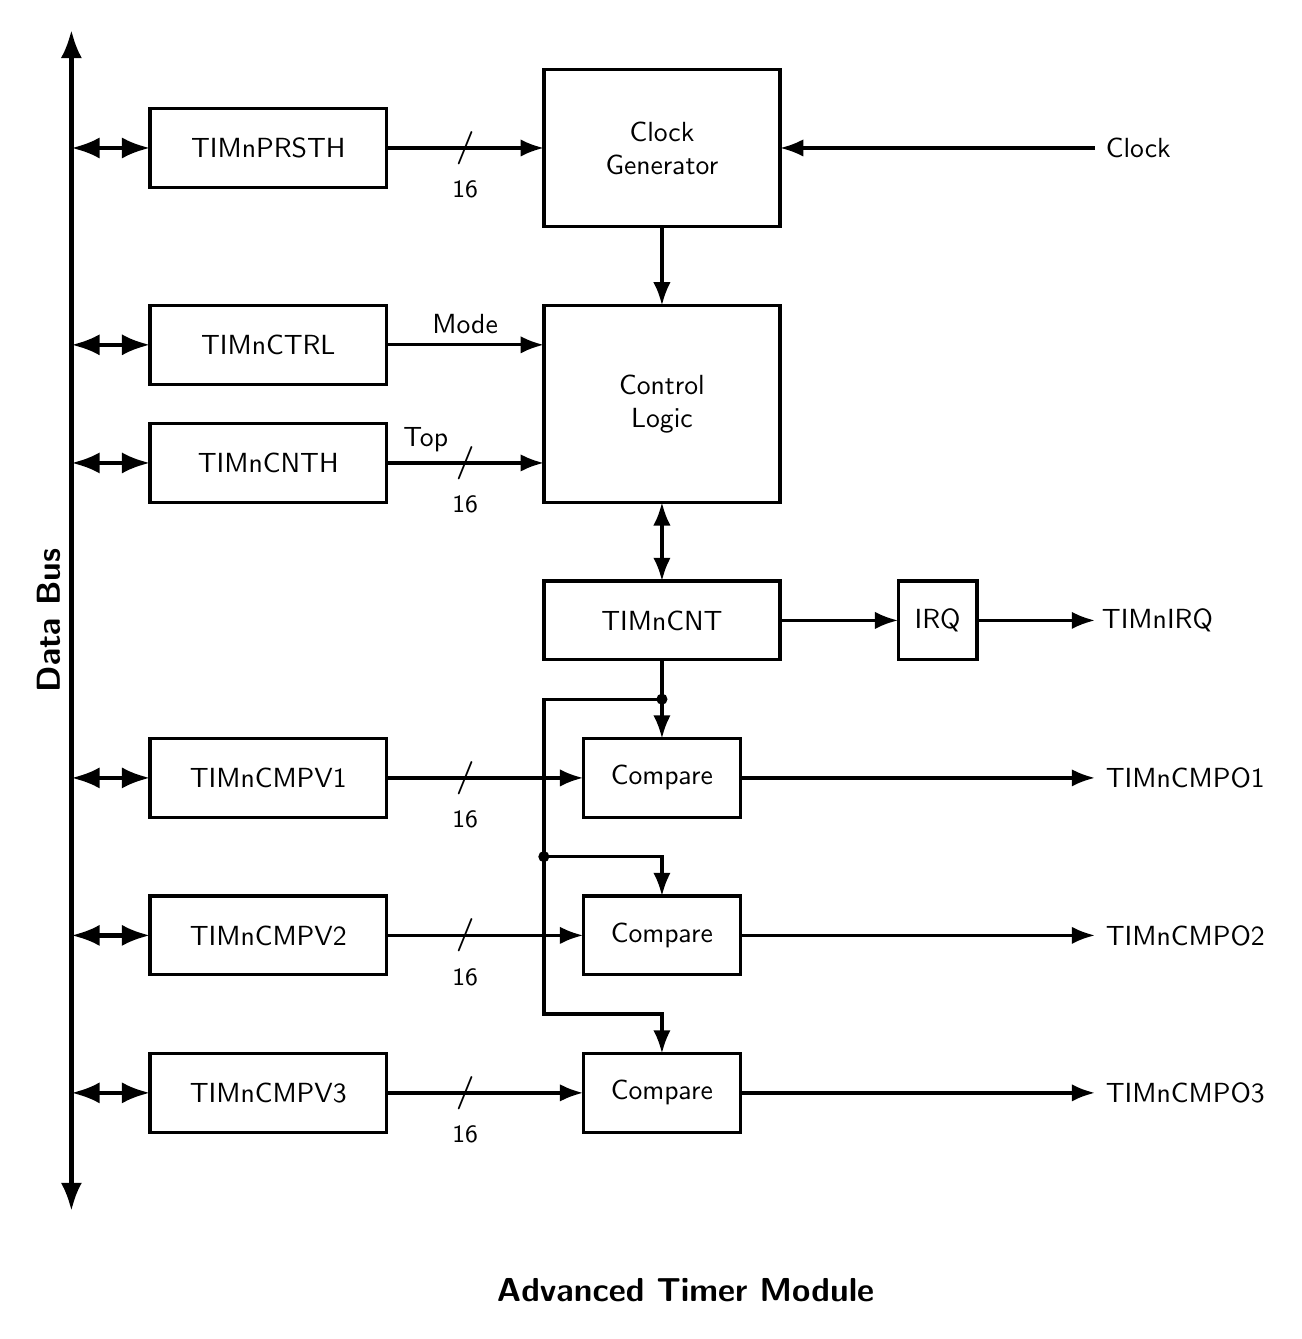
\begin{tikzpicture}[%
		large circuit symbols,
		circuit logic IEC,
		circuit symbol lines/.style={draw, very thick},
		font=\sffamily,
		>=Latex,
		decoration={
          markings,
          mark= at position 0 with {\node[font=\large\bfseries, shift={(1,0)}] {/};}
         }
		]

		%% Hilfslinien. Zeilen auskommentieren, um Hilfslinien zu entfernen!
		
		%\draw [thin,purple,opacity=0.5,step=0.5cm] (0,0) grid (30,20);
		%\draw [purple,opacity=0.5] (0,0) grid (30,20);
		%\foreach \x in {0,...,20} {
	%		\draw [purple] (-0,\x) node[left]{$\x$};
	%		\draw [purple] (30,\x) node[right]{$\x$};
	%	}
	%	\foreach \x in {0,...,30} {
	%		\draw [purple] (\x,20) node[above]{$\x$};
	%		\draw [purple] (\x,0) node[below]{$\x$};
	%	}
		
		\draw[<->, ultra thick] (1, 4) -- node[sloped, anchor=center, above, font=\large\bfseries\sffamily]{Data Bus} (1, 19);
		
		\draw[very thick, font=\sffamily] (2, 18) rectangle (5, 17) node[midway] {TIMnPRSTH};
		\draw[<->, ultra thick] (1, 17.5) -- (2, 17.5);
		
		\draw[very thick, font=\sffamily] (7, 18.5) rectangle (10, 16.5) node[midway, align=center] {Clock\\Generator};
        \draw[->, very thick, postaction={decorate}] (5, 17.5) -- node[below=15pt, anchor=center] {\small 16} (7, 17.5);
        \draw[->, very thick] (8.5, 16.5) -- (8.5, 15.5);
        \draw[->, very thick] (14, 17.5) node[right, align=left, font=\sffamily]{Clock} -- (10, 17.5);
        
        \draw[very thick, font=\sffamily] (7, 15.5) rectangle (10, 13) node[midway, align=center] {Control\\Logic};

        \draw[very thick, font=\sffamily] (2, 15.5) rectangle (5, 14.5) node[midway] {TIMnCTRL};
		\draw[<->, ultra thick] (1, 15) -- (2, 15);
		\draw[->, very thick] (5, 15) -- node[anchor=center, above, font=\sffamily]{Mode} (7, 15);
		
		\draw[very thick, font=\sffamily] (2, 14) rectangle (5, 13) node[midway] {TIMnCNTH};
		\draw[<->, ultra thick] (1, 13.5) -- (2, 13.5);
		\draw[->, very thick, postaction={decorate}] (5, 13.5) -- node[below=15pt, anchor=center] {\small 16} node[anchor=center, above, font=\sffamily, xshift=-0.5cm]{Top} (7, 13.5);
		
		\draw[very thick, font=\sffamily] (7, 12) rectangle (10, 11) node[midway] {TIMnCNT};
		\draw[<->, very thick] (8.5, 13) -- (8.5, 12);
		
		\draw[very thick, font=\sffamily] (11.5, 12) rectangle (12.5, 11) node[midway] {IRQ};
		\draw[->, very thick] (10, 11.5) -- (11.5, 11.5);
		\draw[->, very thick] (12.5, 11.5) node[right, align=right, font=\sffamily, xshift=1.45cm]{TIMnIRQ} -- (14, 11.5);
		
		\draw[very thick, font=\sffamily] (7.5, 10) rectangle (9.5, 9) node[midway] {Compare};
		\draw[very thick, font=\sffamily] (2, 10) rectangle (5, 9) node[midway] {TIMnCMPV1};
		\draw[<->, ultra thick] (1, 9.5) -- (2, 9.5);
		\draw[->, very thick] (8.5, 11) -- (8.5, 10);
		\draw[->, very thick] (8.5, 10.5) node[fill,circle,inner sep=0.5mm]{} -- (7, 10.5) -- (7, 6.5) -- (8.5, 6.5) -- (8.5, 6);
		\draw[->, very thick, postaction={decorate}] (5, 9.5) -- node[below=15pt, shift={(-0.25, 0)}, anchor=center] {\small 16} (7.5, 9.5);
		\draw[<-, very thick] (14, 9.5) node[right, align=left, font=\sffamily]{TIMnCMPO1} -- (9.5, 9.5);
		
		\draw[very thick, font=\sffamily] (7.5, 8) rectangle (9.5, 7) node[midway] {Compare};
		\draw[very thick, font=\sffamily] (2, 8) rectangle (5, 7) node[midway] {TIMnCMPV2};
		\draw[<->, ultra thick] (1, 7.5) -- (2, 7.5);
		\draw[->, very thick, postaction={decorate}] (5, 7.5) -- node[below=15pt, shift={(-0.25, 0)}, anchor=center] {\small 16} (7.5, 7.5);
		\draw[<-, very thick] (14, 7.5) node[right, align=left, font=\sffamily]{TIMnCMPO2} -- (9.5, 7.5);
		
		\draw[->, very thick] (7, 8.5) node[fill,circle,inner sep=0.5mm]{} -- (8.5, 8.5) -- (8.5, 8);
		\draw[very thick, font=\sffamily] (7.5, 6) rectangle (9.5, 5) node[midway] {Compare};
		\draw[very thick, font=\sffamily] (2, 6) rectangle (5, 5) node[midway] {TIMnCMPV3};
		\draw[->, very thick, postaction={decorate}] (5, 5.5) -- node[below=15pt, shift={(-0.25, 0)}, anchor=center] {\small 16} (7.5, 5.5);
		\draw[<->, ultra thick] (1, 5.5) -- (2, 5.5);
		\draw[<-, very thick] (14, 5.5) node[right, align=left, font=\sffamily]{TIMnCMPO3} -- (9.5, 5.5);
		
		\draw (8.8,3) node[align=center]{\large\sffamily\bfseries Advanced Timer Module};
	\end{tikzpicture}
\end{document}
